\section{Implementation}
%     crucial arithmetic
%     How it works together
%     Reference ideas (Maybe from litterature)
%     - Explain how you got th idea
%     - Did you get the idea from somewhere else, explain it from where

% ~10 pages
% -- CHanged as little as possible on reference implementation
% -- Add more automatic testing to compare the changes
% -- Tested with the local reference???

This section will describe how the reference implementation from Bernstein was ported, and how the Karatsuba algorithm is implemented in practice.
\subsection{Reference implementation}
The reference implementation was straight forward to port, as the arithmetic itself could be used directly without any changes. This add confidence that the algorithm is still correct.\medskip
\\
The \texttt{checksum\_compute} function used the \texttt{random\(\)} function given in the C standard library to fill \texttt{p} and \texttt{n} with random values. In the main implementation \texttt{randombytes\(\)} is used to fill \texttt{p} and \texttt{n} with random values, as \texttt{randombytes\(\)} is supplied with the implementation from the rainbowgit implementation\cite{rainbowgit}, 
As the C standard library is not available, an alternative to the \texttt{random\(\)} function is used. Part of the library rainbowgit\cite{rainbowgit} is used for the \texttt{randombytes\(\)} implementation, this implementation uses \texttt{AES} to give a pseudo-random output. As \textit{AES} isn't supplied either, the libcrypto library\cite{libcrypto} is used for its \textit{AES} implementation. It can be found in \textit{src/libcrypto}. It is maintained by the official RISC-V organization, and is actively being developed.

\subsection{Karatsuba algorithm}
To easily allow to enable and disable Karatsuba a C preprocessor definition \texttt{ENABLE\_KARAT} is used. The Karatsuba algorithm will only be included when the definition is present, otherwise it will use the reference implementation.\medskip
\\
The implementation of the algorithm which is described more in theory in subsection \ref{karat-opti} can be explained with a step by step example. In this example the values $2973$ and $3572$ is multiplied. \\
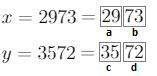
\includegraphics{report/images/karat-split.png}\\
\textbf{Step 1 and 2}, is to compute $a * c$ which is stored in $LOW$ and $b * d$ which is stored in $HIGH$. The recursive step in the code will continue to recursively call itself until the operand length is smaller than the defined \texttt{KARAT\_L}, and the base case is reached and schoolbook multiplication will be used instead.
\lstinputlisting[language=c, firstline=115, lastline=122]{../src/smult.c}
\medskip
\textbf{Step 3} is to compute $(a + b) * (c + d)$ which is stored in $MM$.
\lstinputlisting[language=c, firstline=124, lastline=127]{../src/smult.c}
\medskip
\textbf{Step 4} subtracts the values that was calculated in the last steps. Specifically $MM - LOW - HIGH$, which is stored in $MED$.
\lstinputlisting[language=c, firstline=129, lastline=130]{../src/smult.c}
\medskip
\textbf{Step 5} we simply add $LOW$, $MED$ and $HIGH$, where the numbers have been shifted correctly.
\lstinputlisting[language=c, firstline=132, lastline=134]{../src/smult.c}

\subsection{Testing}
\label{sub-testing}
I wanted to be able to test the code with different values, without having to recompile and restart the emulation every time. The \textit{HAL} library implements a series of serial-functions. Which allows the code to communicate with the host.
\subsubsection{Device}
The embedded device is waiting for the host to send a command, which it acts on. It has 5 different modes that the host can use.
\lstinputlisting[language=c, firstline=19, lastline=23]{../src/test.c}
\medskip
\textbf{MODE\_BLANK} is the default mode. When the device is in \textit{MODE\_BLANK} it waits for a new mode from the host.
\lstinputlisting[language=c, firstline=88, lastline=91]{../src/test.c}
\medskip
\textbf{MODE\_HASH} initializes the \textit{m} and \textit{n} memory with random values, and times the amount of cycles it takes to run \textit{crypto\_scalarmult\_base}. Then sends the \textit{checksum} and \textit{cycles} to the host.
\lstinputlisting[language=c, firstline=51, lastline=67]{../src/test.c}
\medskip
\textbf{MODE\_SEED} takes 48 integers, which is put into the seed memory space, and then the seed is set with \textit{randombytes\_init}.
\lstinputlisting[language=c, firstline=75, lastline=80]{../src/test.c}
\medskip
\textbf{MODE\_PING} is used as part of the initialization of the connection with the test-script on the host. When the host connects to the serial port it sends a \textit{MODE\_PING} command and waits for a reply to ensure the device is listening.
\lstinputlisting[language=c, firstline=70, lastline=72]{../src/test.c}
\medskip
\textbf{MODE\_SET\_KARAT} sets \textit{KARAT\_L} which defines the length of the numbers when the Karatsuba algorithm should use schoolbook multiplication.
\lstinputlisting[language=c, firstline=83, lastline=83]{../src/test.c}
\medskip
\subsubsection{Host}
On the host a test script to connect to the device was written. The script is made in NodeJS\cite{nodejs}, and uses the library SerialPort\cite{serialport} to establish a connection and communicate with the device.
A wrapper function is written to convert the function \textit{port.write(msg, callback)} into a \textit{async} function. 
\lstinputlisting[language=javascript, firstline=15, lastline=18]{../test/index.js}
\medskip
When the connection is opened, the \textit{MODE\_PING} command is sent to the device.
\lstinputlisting[language=javascript, firstline=20, lastline=22]{../test/index.js}
\medskip
As the data from the embedded device is sent in chunks the script needs to be able to detect when a message has been fully received. As a message always ends with \texttt{\}} and then \textit{,} the script will look for thoose two characters to detect when a message has been fully received.
\lstinputlisting[language=javascript, firstline=1, lastline=29]{../test/helpers.js}
The \textit{dataParser} function copies every part of a string into a temporary string, and checks the condition described above. If the message has been received it will return a \textit{JSON} object, otherwise it will return \textit{false}.\medskip
\\
The function \texttt{dataParser} is called when data is received, and only acted upon if if returns a object.  
\lstinputlisting[language=javascript, firstline=28, lastline=31]{../test/index.js}
\medskip
The exsistance of keys on the message object, is used to check what kind of message it is.\\
\medskip
A \textbf{ping} message is received in response to the \textbf{MODE\_PING} sent when the connection is opened. This automatically sets the seed and starts a hash.\\
\medskip
The \textbf{checksum} message is received when a hash iteration is successful, which just prints out the message and replies with the \textbf{MODE\_HASH} mode.
\label{karatTesting}
If the variable \textit{karaI} is set to a number, then it tries to iterates over all "breaking" points for what length to use the schoolbook multiplication instead of the Karatsuba algorithm. It does this by waiting for \textbf{ping} and \textbf{checksum} messages, and trying every value up until 64, and saving the cycles result for every value.
\lstinputlisting[language=javascript, firstline=34, lastline=55]{../test/index.js}
